\chapter{Implementation
    \label{chapter:implementation}}

This chapter describes the tools, methods, and rationale behind the implementation. 
As mentioned earlier, based on initial tests, CLIP and TinyCLIP were selected as the models for this work.


\section{Model Acquisition}

The CLIP models were sourced from the official CLIP GitHub repository \cite{clipgit}.
Similarly, the TinyCLIP models were obtained from the official TinyCLIP GitHub repository \cite{tinyclipgit}.
Alternatively, models can be retrieved from HuggingFace \cite{huggingface}.
However, the challenge with HuggingFace is that the models cannot be split into separate image and text encoders.
For this reason, only models from the official CLIP and TinyCLIP repositories were used.
The API to use these network is self explainatory.
The implementaion is done with Pytorch\cite{pytorch}.
In \cref{methods:tab:clipsize}, the parameter count for all CLIP and TinyCLIP implementations using a ResNet as the image encoder is provided.
It is evident that TinyCLIP uses significantly fewer parameters than the original CLIP.

\section{Model Translation
\label{implementation:sec:translation}}

The models were first split into separate image and text encoders.
The image encoder is converted into an ONNX graph, which is then simplified.
To get the ONNX graph the ONNX exporter from Pytorch is used.
This ONNX graph is later translated by the \acrshort{dfc} into \acrshort{har} and \acrshort{hef} files.
The \acrshort{dfc} needs a \acrshort{gpu} to perform some tasks or just to speed up compilation.
Due to the fact that no \acrshort{gpu} was available for this project, not all of the \acrshort{dfc} features were used.
The model weights are quantized to 8 bits.


\begin{figure}
    \centering
    \subfloat[End of CLIP ResNet50x4 vision encoder ONNX graph acquired through official CLIP]{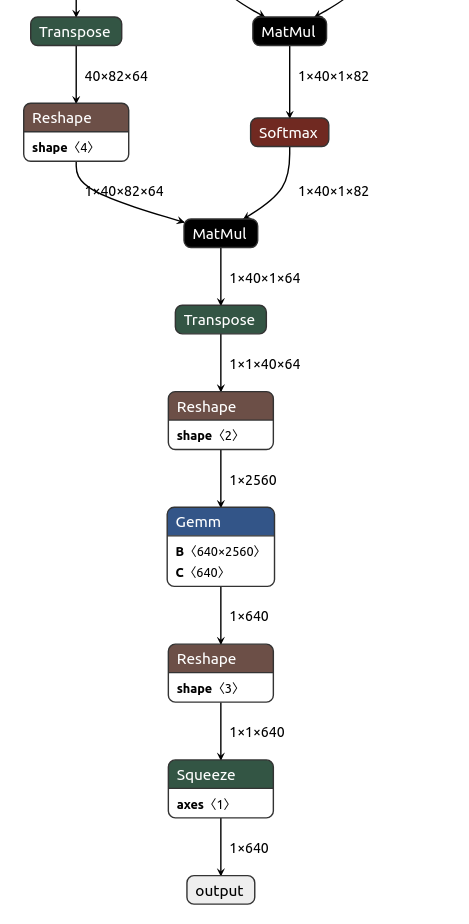
\includegraphics[width=0.4\textwidth]{Images/Implementation/ClipRes50x4.png}\label{fig:implementation:clipres50x4}}
    \qquad
    \subfloat[End of CLIP ResNet50x4 vision encoder ONNX graph sent by Hailo]{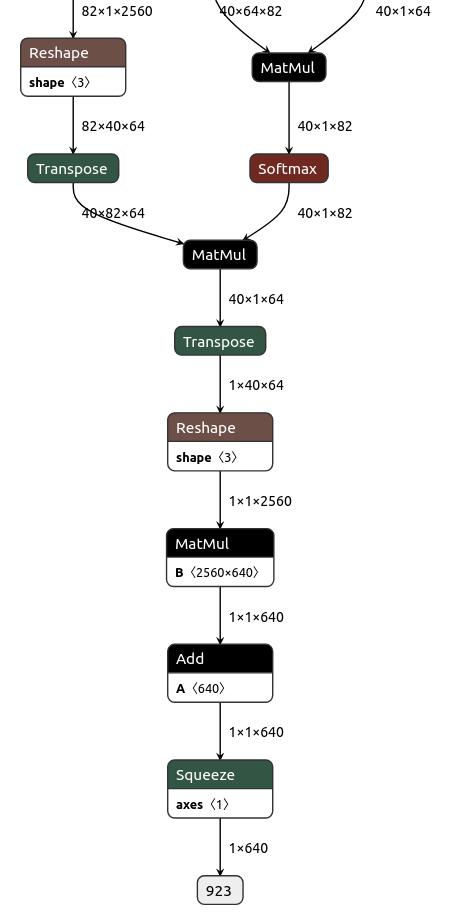
\includegraphics[width=0.4\textwidth]{Images/Implementation/HailoClipRes50x4.png}\label{fig:implementation:hailoclipres50x4}}
    \caption{Comparison of CLIP ResNet50x4 vision encoder ONNX graph (a) from official CLIP and (b) from Hailo. The key difference is in the number of dimensions.}
    \label{fig:implementation:compareRN50x4}
\end{figure}

\subsection{Splitting the Graph}

The first major issue encountered during the translation step is that the \acrshort{dfc} cannot compile Transformers.
Specifically, the problem arises from a transpose block at the end of every self-attention layer.
The \acrshort{dfc} swaps dimensions and combines the last two dimensions, leading to conflicts.
In the ResNet model obtained through the official CLIP repository (see \cref{fig:implementation:clipres50x4}), the transpose block after the MatMul block swaps the second and third dimensions.
This results in a compilation error because the \acrshort{dfc} has already combined the last two dimensions.

This behavior was discussed with Hailo, and they provided an example where CLIP is run on their hardware. Upon testing, it is observed that the error does not occur when using the model provided by Hailo.
The reason for this discrepancy is that the networks used by Hailo were acquired with an older version of CLIP and the ONNX exporter.
The attempt to recreate the graph from hailo failed due to version dependencies.
While the graphs are functionally equivalent, the architecture differs slightly.
As seen in \cref{fig:implementation:hailoclipres50x4}, the model provided by Hailo has a maximum of three dimensions.
To work around this problem, the ONNX graph is cut off between the last matmul and transpose block.
For this task, the Onnx-Modifier tool \cite{onnxmodifier} is used.
The removed graph are implemented as postprocessing steps.
After quantization, the graph can again be visualized using a tool called Profiler from Hailo.
In \cref{fig:implementation:compareRN50x4qunathar}, the compiled model with the cutoff end is visualized.
In this figure, the combination of the last dimensions can be seen.

\begin{figure}
    \centering
    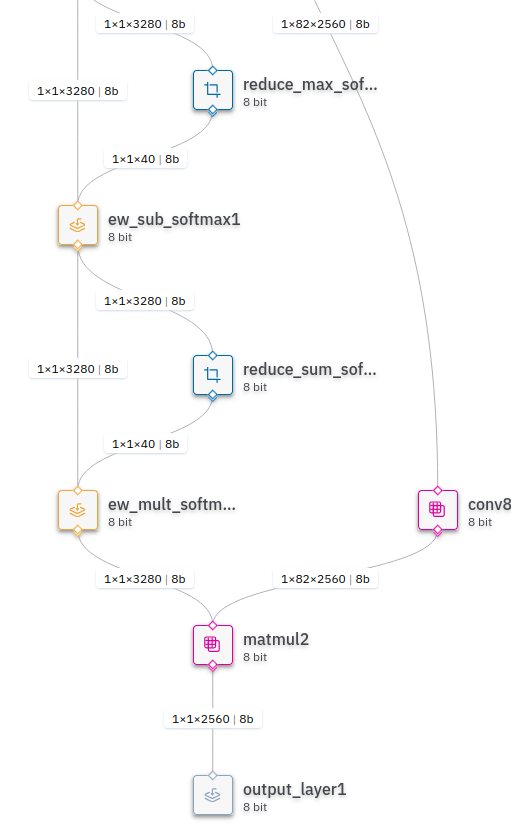
\includegraphics[width=0.4\textwidth]{Images/Implementation/ClipRes50x4_qunat_Har.png}
    \caption{Output of the \acrshort{dfc} after compiling the modified ONNX graph of the ResNet50x4.}
    \label{fig:implementation:compareRN50x4qunathar}
\end{figure}

This graph is then compiled into a \acrshort{hef} file, which can be executed on the Hailo hardware.
To use CLIP, the text embeddings are also required.
Due to the limitation that Transformers cannot be used with Hailo, the embeddings are calculated on a PC and saved in a JSON file.
The JSON format is used because it is readable.

\subsection{Rest of the Graph}

As mentioned earlier, the cut-off part of the ONNX graph is handled during post-processing. 
The cut-off part consists of a matrix multiplication and some reordering of dimensions. 
In the first implementation, the weights for the matrix multiplication were extracted and saved in a JSON file.
In a second attempt, the cut-off ONNX graph was used directly.
The second attempt proved to be faster and used less memory.
The cut location can be seen in \cref{fig:implementation:RNcut}.

\begin{figure}
    \centering
    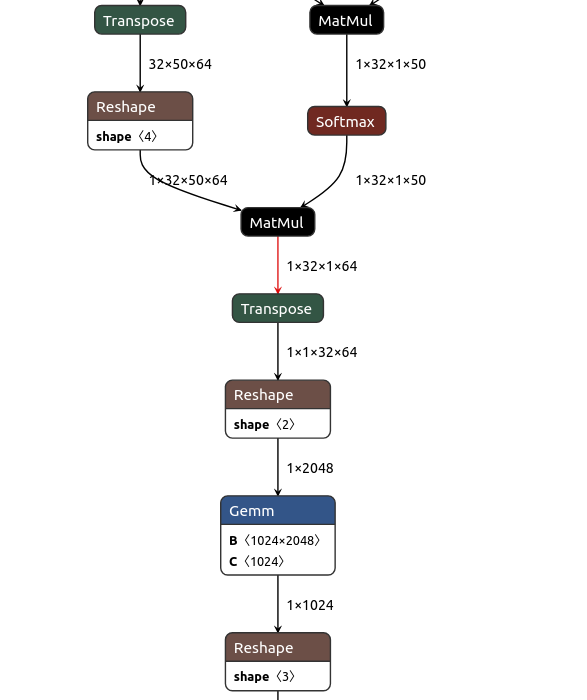
\includegraphics[width=0.4\textwidth]{Images/Implementation/firstcutlocation.png}
    \caption{Graph for the RN50. The Cut is made at the red arrow between the MatMul and the Transpose block.
    The location is similar for all models.}
    \label{fig:implementation:RNcut}
\end{figure}
\section{Inference}

To ensure a fair comparison of performance, the implementation on the Raspberry Pi closely mirrors the one used on the PC. 
The PC application follows a similar structure to the one used by Lia Winkler in her work.
The application calculates the probability score for indoor / outdoor, all outdoor subclasses and all indoor subclasses.
After that the score are evaluated.
First the distinction between indoor and outdoor is made by comparing the corresponding scores.
Then either the indoor subclasses or the outdoor subclasses are evaluated to finaly classify the image.
This process can be seen in \cref{fig:overview:evaluation}.
There the evaluation for the Raspberry Pi is showed.
On PC the text embeddings are directly calculated with the text encoder.

Due to the limitations of the \acrshort{dfc}, only ResNets are used as the image encoder.
To utilize a model on Hailo, the Python API is employed. 
Two different implementations were tested.

The first implementation is based on a code snippet found in \cite{hailoimplementation}.
In this implementation, the device is initialized every time an output is calculated, which significantly slows down the program and results in no substantial speedup.

The second implementation addresses this issue by initializing the device once at the start of the program. 
The template for this attempt is taken from the \cite{hailo_application_code_examples}.
There the code for the detection pipeline example is taken as a baseline.

\subsection{Text Input}

For the text input, the subclasses from \cref{tab:dataset:subclasses} are used. 
These subclasses are wrapped in sentences and then used as input for the text encoder.
In \cite{clip}, the authors state that the performance of the network can improve if the text inputs are framed within sentences.
The used sentences look like this:
\begin{itemize}
    \item A photo of a \dots
    \item A picture of a \dots
    \item An image of a \dots
    \item A \dots scene
    \item A picture showing a scene of a \dots
\end{itemize}
The output from the text encoder, the text embeddings, are then saved in a JSON file.

\subsection{Image Input}
The Hexagon dataset is used as image input.
It consists of panorama images. 
These images are divided into 5 equal-sized patches, and each patch is processed with CLIP.
To process one of these patches with CLIP, it must first undergo pre-processing by resizing it to the required input size.
The pre-processing steps consist of the following:

\begin{itemize}
    \item Resize (to for example \(244 \times 244\) pixel)
    \item Center-crop
    \item If not already in RGB, convert the image to RGB
    \item Normalize to mean 0 and standard deviation 1
\end{itemize}

Mean and standart deviation for normalization are calculated over the entire Hexagon dataset.
These steps are included natively in any pre-process for CLIP or CLIP-like networks.
Finally, a majority vote is taken over the subclasses of the patches to classify an image. 
This process, mentioned in Lia Winkler's report, helps improve the accuracy of the predictions.

\section{Evaluation}

To measure the performance of the Hailo hardware, the models were tested in three different environments:
\begin{itemize}
    \item CPU on PC (Intel Core i7-14700)
    \item CPU on Raspberry Pi 5
    \item Hailo-8L entry level hardware accelerator
\end{itemize}
The implementations were made as similar as possible to ensure the values are correct and representative. 

The following metrics were used to measure performance:
\begin{itemize}
    \item Throughput (speed)
    \item Accuracy
    \item Size (parameter count and Memory)
\end{itemize}

For throughput, two measurements were taken:
The first measures the time from input to output, including calculating the text embeddings, the image embeddings, and the dot product of the embeddings. This measurement is called throughput and is measured in iterations per second (it/s).
The second measures the time it takes to calculate one image embedding. This measurement is called throughput image and is also measured in iterations per second (it/s).
Both measurements are calculated on a subset of 100 images.

Accuracy describes how well a model performs in labeling images.
It is calculate by dividing the correctly classified images by the total amount of images.
This metric is useful for checking if a network works correctly, but it may be misleading because it does not account for unbalanced datasets.
In order to make a more precise statement, balanced accuracy is used.
Balanced accuracy takes the amount of data from a class in consideration.
The confusion matrices to all model evaluations are provided in the appendix.
In the text, accuracy is also used to refer to the models ability to classify images correctly.

Although the Raspberry Pi has ample memory, it is always good practice to consider the size of a model as a metric. Size is measured in terms of memory or parameter count.

\subsection{Without Hardware Accelerator}
In \cref{methods:tab:perfPC}, the performance on a PC CPU is displayed. These values are used to compare the performance with the Hailo hardware accelerator.

\begin{table}[tbp]
    \centering
    \begin{tabular}{l|rrrrr}
    \hline
        Model Name & Accuracy & \makecell{Balanced \\accuracy}&\makecell{Throughput\\(it/s)} & \makecell{Throughput \\ Image (it/s)} \\ \hline
        RN50 & 0.845& 0.596& 12.46 $\pm$ 5.33& 32.48 $\pm$ 3.18 \\ 
        RN50x4 & 0.937& 0.856& 5.79 $\pm$ 2.04& 12.13 $\pm$ 0.86 \\ 
        RN50x16 & 0.870& 0.889& 2.51 $\pm$ 0.55& 3.81 $\pm$ 0.17 \\ 
        RN50x64 & 0.939& 0.855& 0.88 $\pm$ 0.11& 1.13 $\pm$ 0.03\\
        RN101 & 0.882& 0.706& 9.38 $\pm$ 3.43& 20.01 $\pm$ 1.81\\  
        TinyCLIP-19M & 0.805& 0.830&54.06 $\pm$ 8.37& 20.38 $\pm$ 3.65 \\ 
        TinyCLIP-30M & 0.839& 0.822&37.53 $\pm$ 5.72& 13.59 $\pm$ 3.31 \\ 
    \end{tabular}
    \caption{Performance table from evaluation on PC CPU.}
    \label{methods:tab:perfPC}
\end{table}

In \cref{methods:tab:perfRaspi}, the performance measurements from executing on the Raspberry Pi CPU are displayed. RN50x16 and RN50x64 are missing because they are too large to evaluate on the Raspberry Pi.

As expected, the throughput on the Raspberry Pi is significantly lower than the throughput on the PC CPU from \cref{methods:tab:perfPC}, due to the lower computing power of the Raspberry Pi. In a first test, the accuracy from the Raspberry Pi CPU differd slightly from the PC.
A first suspision was that this is due to different CPU architecture.
Later an error in the evaluation was found where the 5 patches were not sorted.
This means that 5 patches that did not belong to the same image were evaluated together.
This error is present in the code taken from Lia Winkler.

In \cref{methods:tab:perfRaspi}, the parameter count of the image encoder is displayed. These values are the same for the models on both the PC and the Raspberry Pi.


\begin{table}[]
    \centering
    \begin{tabular}{l|rrrrr}
    \hline
    Modelname & Accuracy &  \makecell{Balanced \\accuracy}&\makecell{Throughput\\(it/s)} & \makecell{Throughput \\ Image (it/s)} & \\ \hline
        RN50 & 0.845 & 0.596 & 1.15 $\pm$ 0.36 & 2.85 $\pm$0.05 \\ 
        RN50x4 & 0.937 & 0.856 & 0.61 $\pm$ 0.14 & 1.13 $\pm$ 0.016\\
        RN101 & 0.882 & 0.706 & 0.92 $\pm$ 0.24 & 1.89 $\pm$ 0.038\\  
        TinyCLIP-19M & 0.805 & 0.830 & 2.27 $\pm$ 0.63& 5.22 $\pm$ 0.16\\ 
        TinyCLIP-30M & 0.839 & 0.822 & 1.60 $\pm$ 0.47& 3.79 $\pm$0.09\\ 
    \end{tabular}
    \caption{Performance evaluation on Raspberry Pi CPU.}
    \label{methods:tab:perfRaspi}
\end{table}



\begin{table}[]
    \centering
    \begin{tabular}{l|rrr}
    \hline
    Model name & \begin{tabular}[c]{@{}l@{}}Parameters\\ Visual (Mio)\end{tabular} & \begin{tabular}[c]{@{}l@{}}Parameters\\ Text (Mio)\end{tabular} & \begin{tabular}[c]{@{}l@{}}Parameters\\ \acrshort{har} quantized (Mio)\end{tabular} \\ \hline
    RN50                & 38.3  & 37.8  &36.2\\
    RN50x4              & 87.1  & 59.1  &85.3\\
    RN50x16             & 167.3 & 850.5 & -\\
    RN50x64             & 420.4 & 151.1 & -\\
    RN101               & 56.3  & 37.8  &55.1\\
    TinyCLIP-19M        & 18.5  & 18.9  &17.1\\
    TinyCLIP-30M        & 29.5  & 28.3  &27.7\\ 
    \end{tabular}
    \caption{Parameter count for different CLIP and TinyCLIP implementations with ResNet as the visual encoder.}
    \label{methods:tab:clipsize}
\end{table}




\subsection{With Hardware Accelerator}

Now, the networks after compilation are examined.
First, the number of parameters in the compiled \acrshort{har} file is analysed.
There is a slight decrease in the number of parameters, which can be explained.
In the case of TinyCLIP-19M, the cut-off graph is composed of a matrix multiplication with a matrix of the shape \(1024 \times 1408\).
With the following calculation:

\begin{equation*}
    1024 \times 1408 + 1024 = 1'442'816
\end{equation*}

the parameter count for the cut-off graph is obtained. Now, this is added to the parameter count of the model, resulting in:

\begin{equation*}
    1.4 \text{M} + 17.1 \text{M} = 18.5 \text{M} 
\end{equation*}

which is the parameter count before compilation (see \cref{methods:tab:clipsize}).
This calculation can also be done for all other models, but the result is the same.
This result means that the all parameters are used, indicating that no changes to the architecture were made in the compilation of the \acrshort{har} files.


\subsection{Model Size Comparison}

In \cref{methods:tab:sizecompare}, a comparison between the file sizes of ONNX and HEF models after compilation for various CLIP configurations is presented.
As expected, the ONNX models are significantly larger due to the higher precision (FP32), while the HEF files, which are quantized to INT8, are smaller.
This size reduction is a direct result of the \acrshort{dfc}'s quantization process.
For example, the model RN50 has a file size of 153.2 MB in ONNX format, but after being compiled to HEF, it reduces to 53.7 MB.
Similar reductions in size can be observed for other models such as RN50x4, RN101, TinyCLIP-19M, and TinyCLIP-30M.
Because of quantization, the memory size should be around 4 times lower than before, as the datatype of the weights changes from FP32 to INT8.
In reality, the factor is around 3.
It is important to mention that these numbers should be taken with a grain of salt because the datatypes of the saved models are different.
This reduction improves memory efficiency when deploying these models on hardware accelerators like Hailo.

\begin{table}
    \centering
    \begin{tabular}{l|rr}
    \hline
    Modelname & Onnx & \acrshort{hef}\\\hline
    RN50 & 153.2 MB & 53.7 MB \\ 
    RN50x4 & 348.4 MB & 121.7 MB  \\ 
    RN101 & 224.9 MB  & 82.7 MB \\
    TinyCLIP-19M & 74.3 MB & 28.6 MB  \\ 
    TinyCLIP-30M & 118.3 MB & 43.5 MB  \\ 
    \end{tabular}
    \caption{Comparison in size between ONNX and HEF file of a CLIP model.}
    \label{methods:tab:sizecompare}
\end{table}

\begin{table}[]
    \centering
    \begin{tabular}{l|rrrrr}
    \hline
    Modelname & Accuracy &  \makecell{Balanced \\accuracy}&\makecell{Throughput\\(it/s)} & \makecell{Throughput \\ Image (it/s)} & \\ \hline
    RN50 & 0.799 & 0.200 & 20.63 $\pm$ 1.34 & 24.58 $\pm$ 0.27  \\ 
    RN50x4 & 0.840 & 0.419 & 10.13 $\pm$ 0.32 & 10.75  $\pm$ 0.059\\
    RN101 & 0.784& 0.514 & 15.61 $\pm$ 0.49 & 17.09 $\pm$ 0.081\\  
    TinyCLIP-19M & 0.088 & 0.200 & 30.41 $\pm$ 2.71 & 39.29 $\pm$ 3.02 \\ 
    TinyCLIP-30M & 0.574 & 0.536 & 22.96$\pm$ 1.57 & 27.82 $\pm$ 1.71\\ 
    \end{tabular}
    \caption{Performance table from evaluation on Hailo 8L.}
    \label{methods:tab:perfHailo}
\end{table}

\subsection{Speed and Accuracy Analysis}

Now, let's examine the performance in terms of speed and accuracy.
In \cref{methods:tab:perfHailo} the performance metrics for models evaluated on the Hailo-8L hardware accelerator are presented.
Notably, the throughput on the Hailo device is much higher compared to the Raspberry Pi CPU (see \cref{methods:tab:perfRaspi}).

On first glance, it appears that accuracy only drops for the TinyCLIP models.
However, a closer look reveals that the accuracy of the ResNet models may also be misleading.
To understand the true performance, the confusion matrix for the RN50 model (see \cref{methods:fig:compareConfM}) and the balanced accuracy as a measurement are used.
In \cref{methods:tab:perfRaspi} a pattern appears.
The models which original have a low parameter count lose much of their accuracy after quantization.
This effect can be seen with RN50 and TinyCLIP-19M.
TinyCLIP-19M has the biggest drop in accuracy of more then 60\%.


\begin{figure}[!h]
    \centering
    \subfloat[][Evaluation on PC]{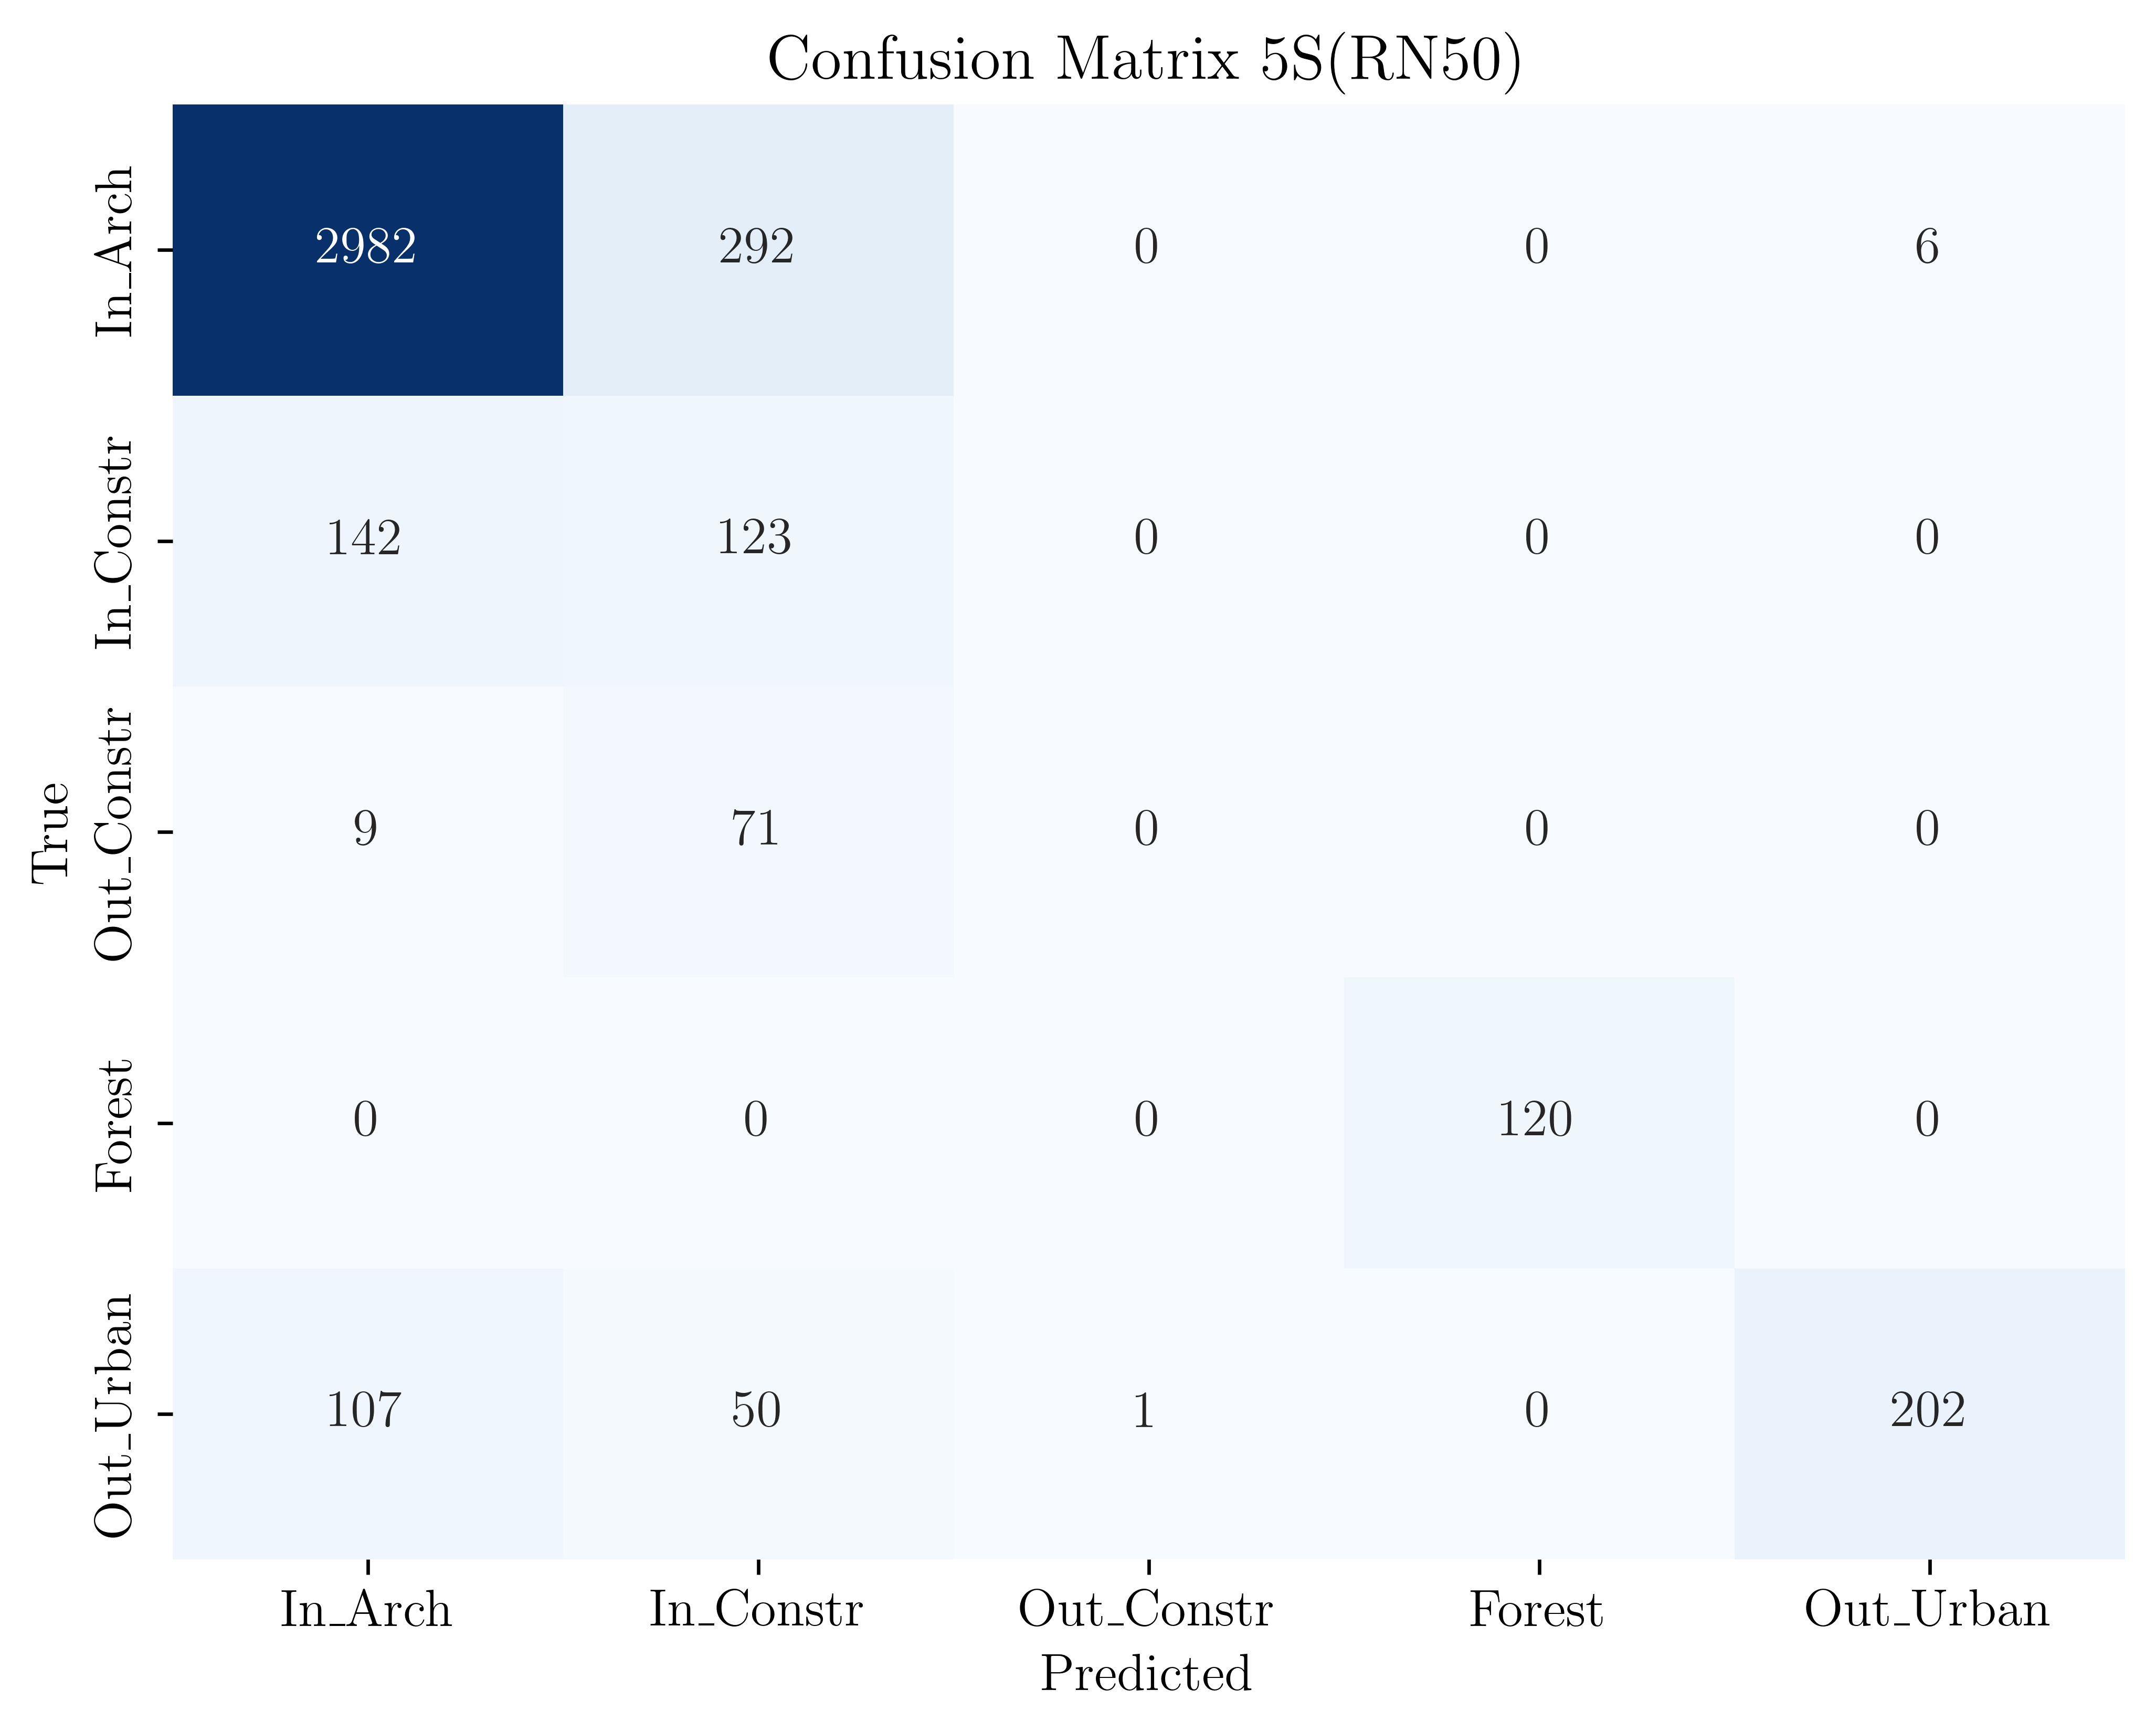
\includegraphics[width=0.49\textwidth]{Images/appendix/resultsPC/Confusion Matrix 5S(RN50).png}\label{methods:fig:confrn50pc}}
    \subfloat[][Evaluation on Hailo]{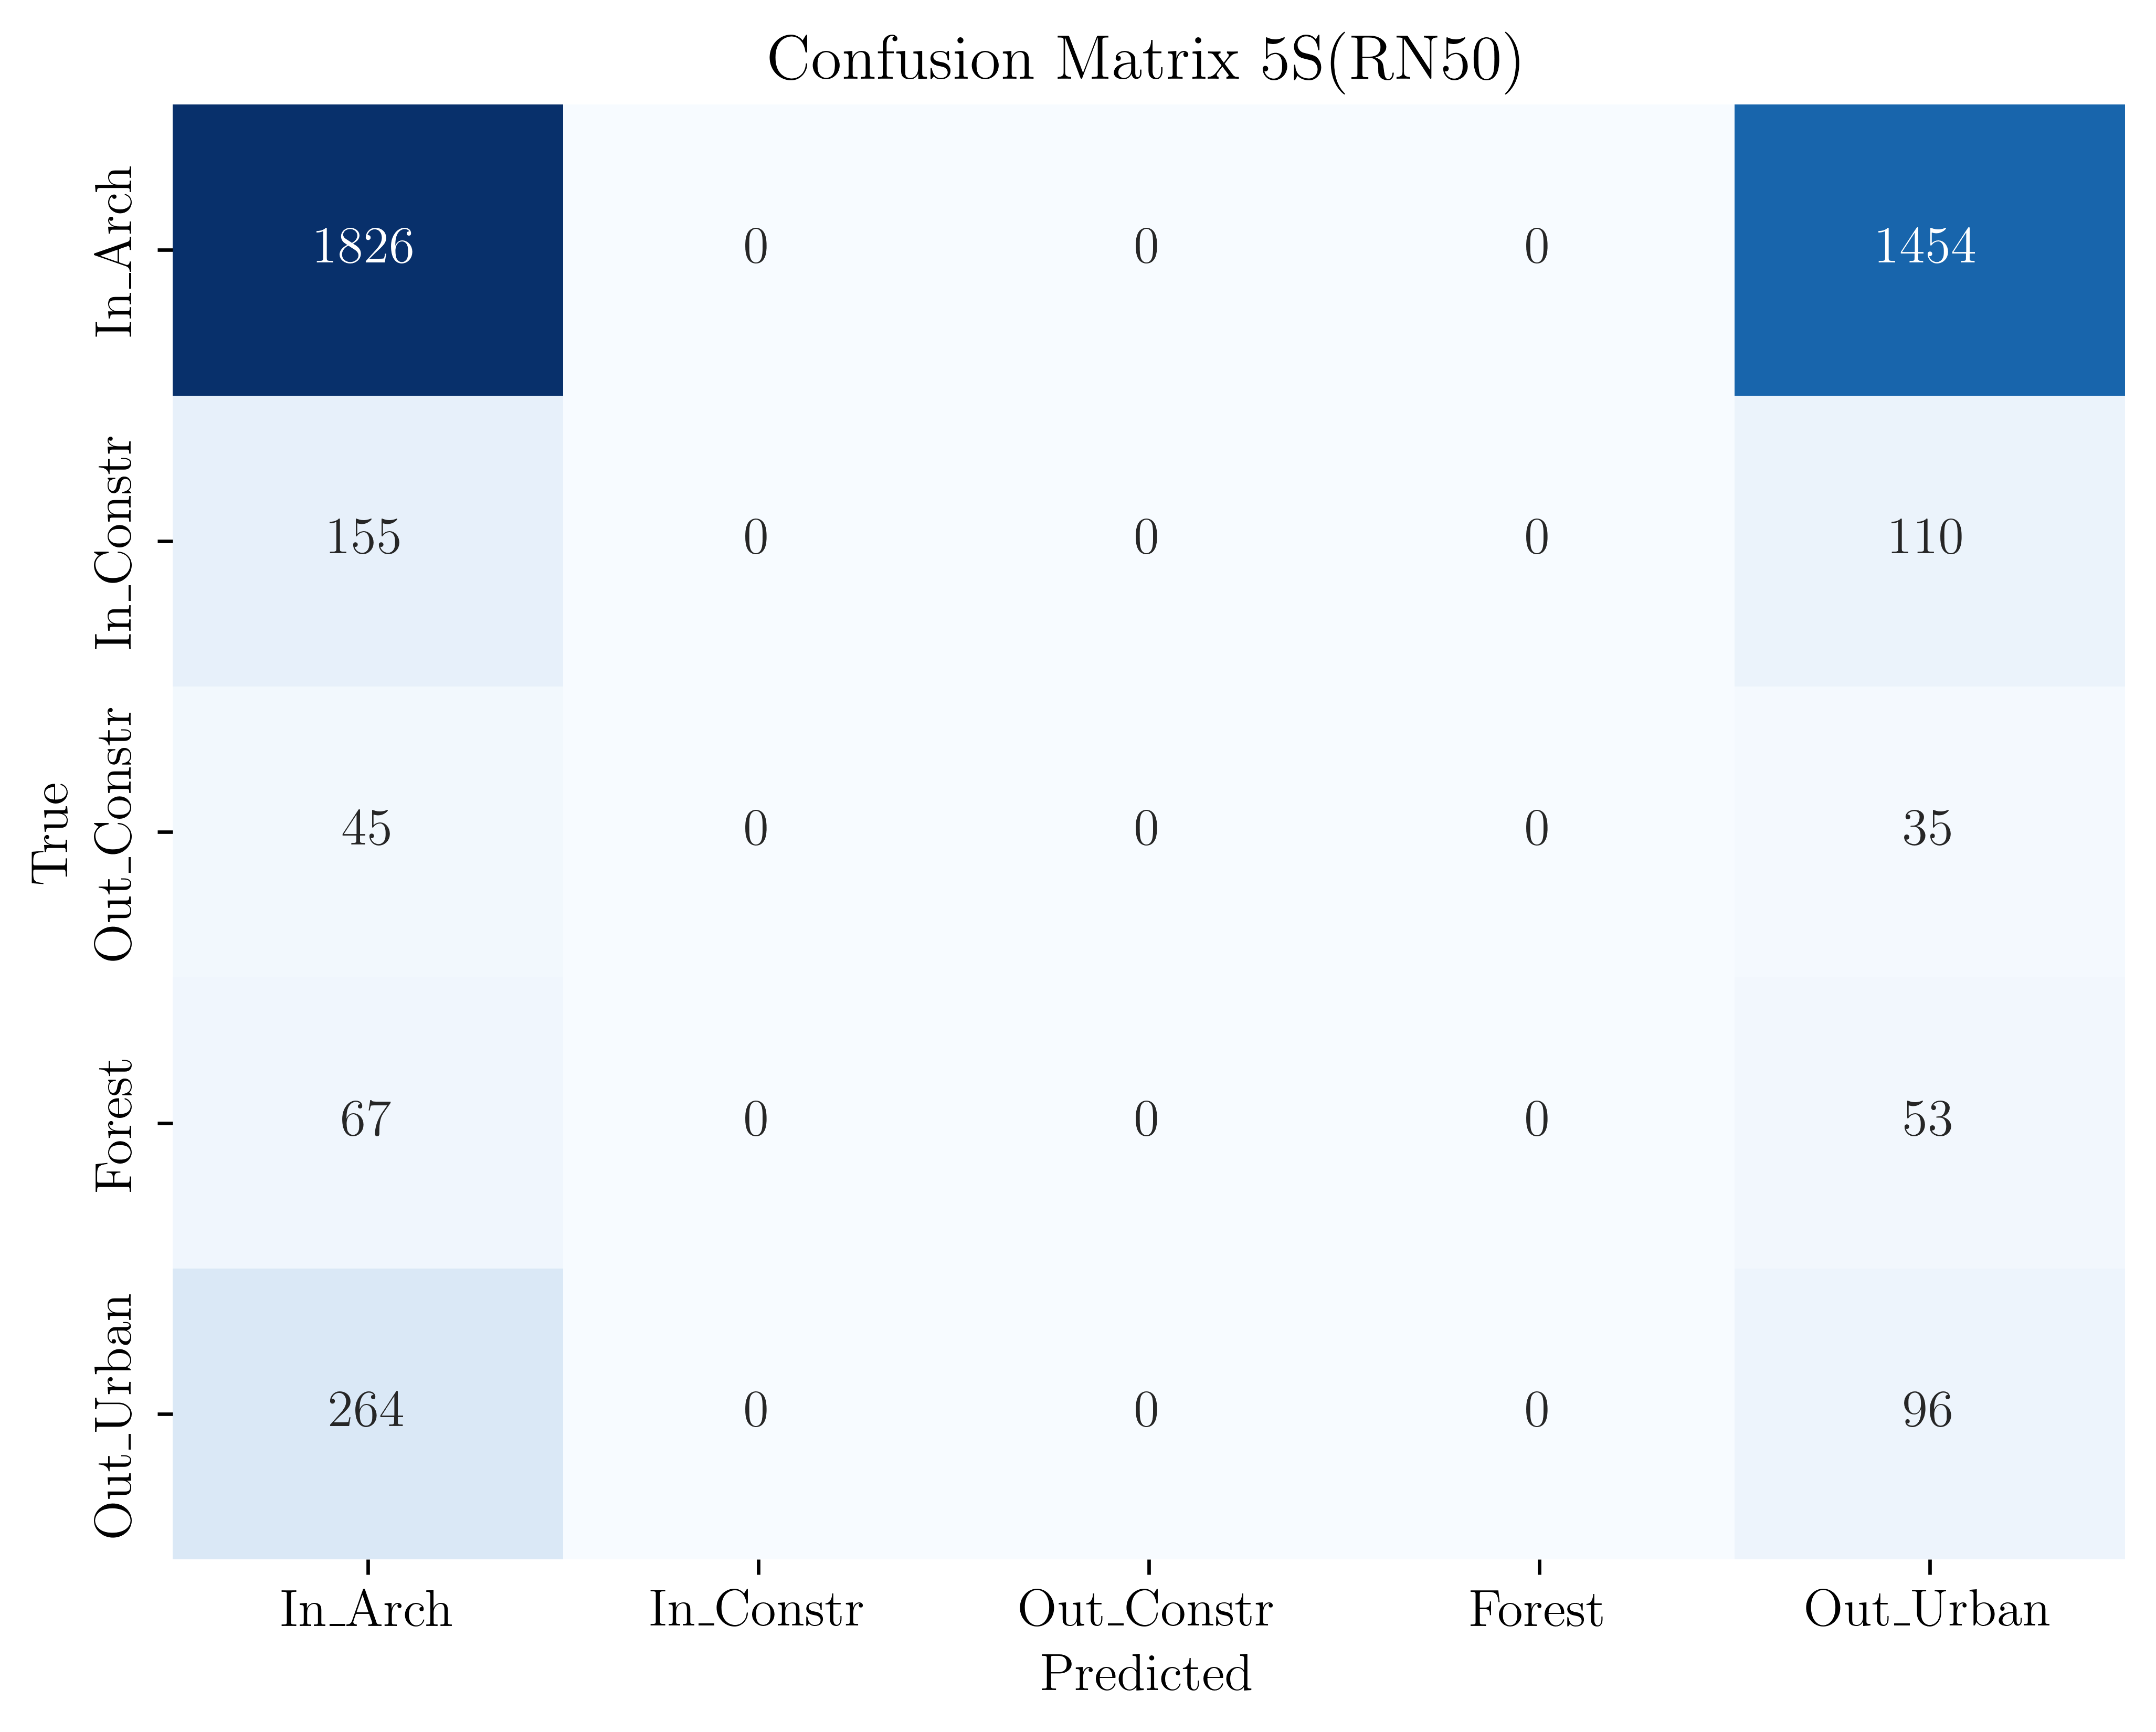
\includegraphics[width=0.49\textwidth]{Images/Implementation/Confusion Matrix 5S(RN50)Hailo.png}\label{methods:fig:confrn50hailo}}
    \label{methods:fig:compareConfM}
    \caption{Comparison of confusion matrix from Hailo to PC.}
\end{figure}

There are several possible reasons for the discrepancies between the PC and Hailo evaluations, which are reflected in the balanced accuracy:
\begin{itemize}
    \item \textbf{Bad Quantization:} The model's performance could be degraded due to suboptimal quantization, which may result in incorrect classification of the images.
    \item \textbf{Implementation Errors:} There could be a mistake in the implementation, such as errors in the creation of the confusion matrix or during post-processing.
    \item \textbf{Differences in Text Embeddings:} The text embeddings used by the models could differ between platforms, affecting the classification accuracy.
\end{itemize}

\section{Control Implementation
    \label{scetion:methods:contimp}}

The first step in identifying the issue is verifying the creation of the confusion matrix.
Since the same code is used on both Hailo and PC the consistency of the outputs can be checked.
The model outputs are saved to a CSV file, and after comparison, it was confirmed that the confusion matrix generated on Hailo matches the one computed on the PC.

Next the text embeddings are checked.
As mentioned earlier, the text embeddings are saved in a JSON file.
Possible errors could arise from incorrect saving or rounding of the embeddings during the process.
To verify this, the output of the text encoder with the corresponding JSON file were compared.
In all cases, the differences were found to be zero, indicating that the embeddings were identical across both platforms.

\begin{figure}[h]
    \centering
    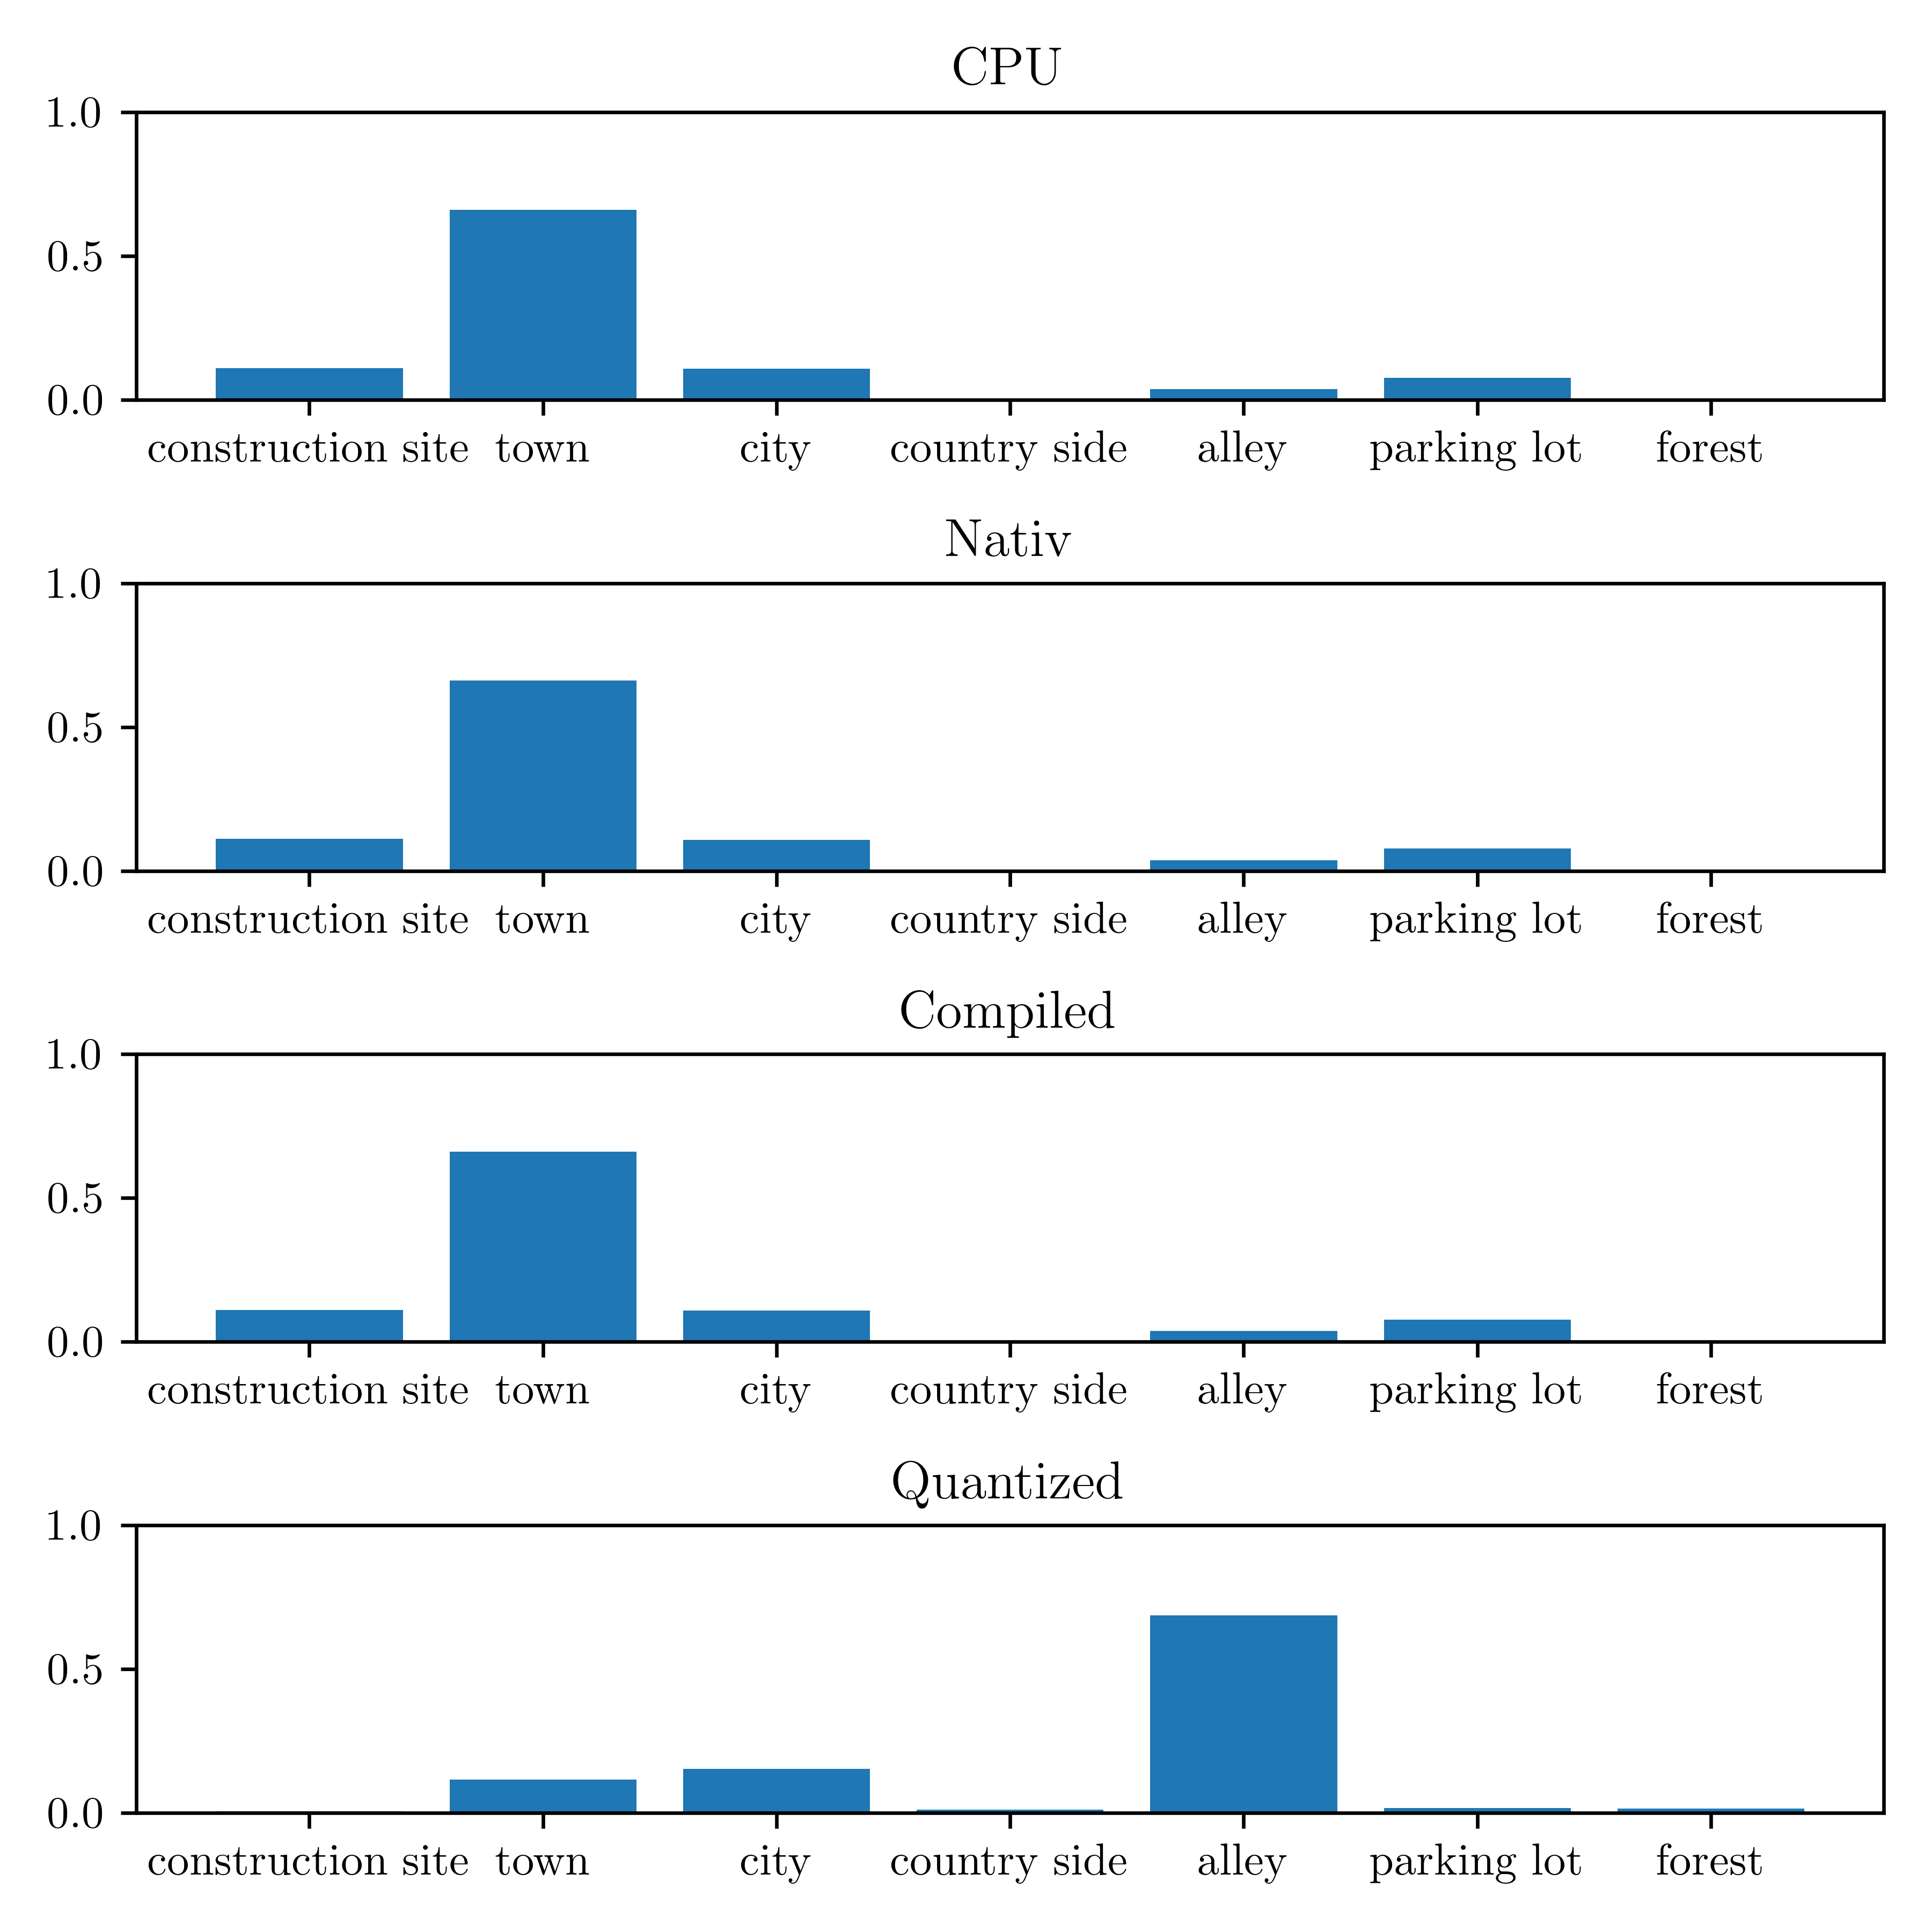
\includegraphics[width=0.6\textwidth]{Images/Implementation/compareProbs_RN50.png}
    \caption{Compare outputs at different \acrshort{dfc} points with RN50.}
    \label{methods:fig:comparern50}
\end{figure}

To check the functionality, the output and of the quantization the output of the \acrshort{dfc} is checked at every stage.
The \acrshort{dfc} is able to calculate the output of the compiling network at every step.
With that the postprocessing and the functionality of the quantization can be checked.
The test is conducted with a test image (see \cref{methods:fig:comparetestpic}).
The Results can be seen in \cref{methods:fig:comparern50}.
It can be seen that the output from CPU, Nativ and Compiled are the same.
Nativ is the model which results in the translation from onnx to \acrshort{har}.
Compiled is floating point omptimized by the \acrshort{dfc}.
This result confirms that postprocessing is implemented correct otherwise the nativ output would be different from the CPU output.
After quantization there is a huge shift of the output.
The effect can also be seen on the output of other images.
This indicates that the quantization is the problem.

Important to mention is that in the process of creating the \acrshort{hef} file changes to the model architecture can happen in the form of 
layer fusion and memory optimization.
The effect of these changes can be seen in \cref{methods:fig:comparern50harhef} where the output of the quantized \acrshort{har} file is different from the output from the output calculated on Hailo with the compiled \acrshort{hef} file.
This effect makes it diffcult to make a precise statment about the state of quantization.
A similiar effect can be seen on the \acrshort{har} output compared to the \acrshort{hef} output as in both ouput "alley" has the highest probability.

\begin{figure}
    \centering
    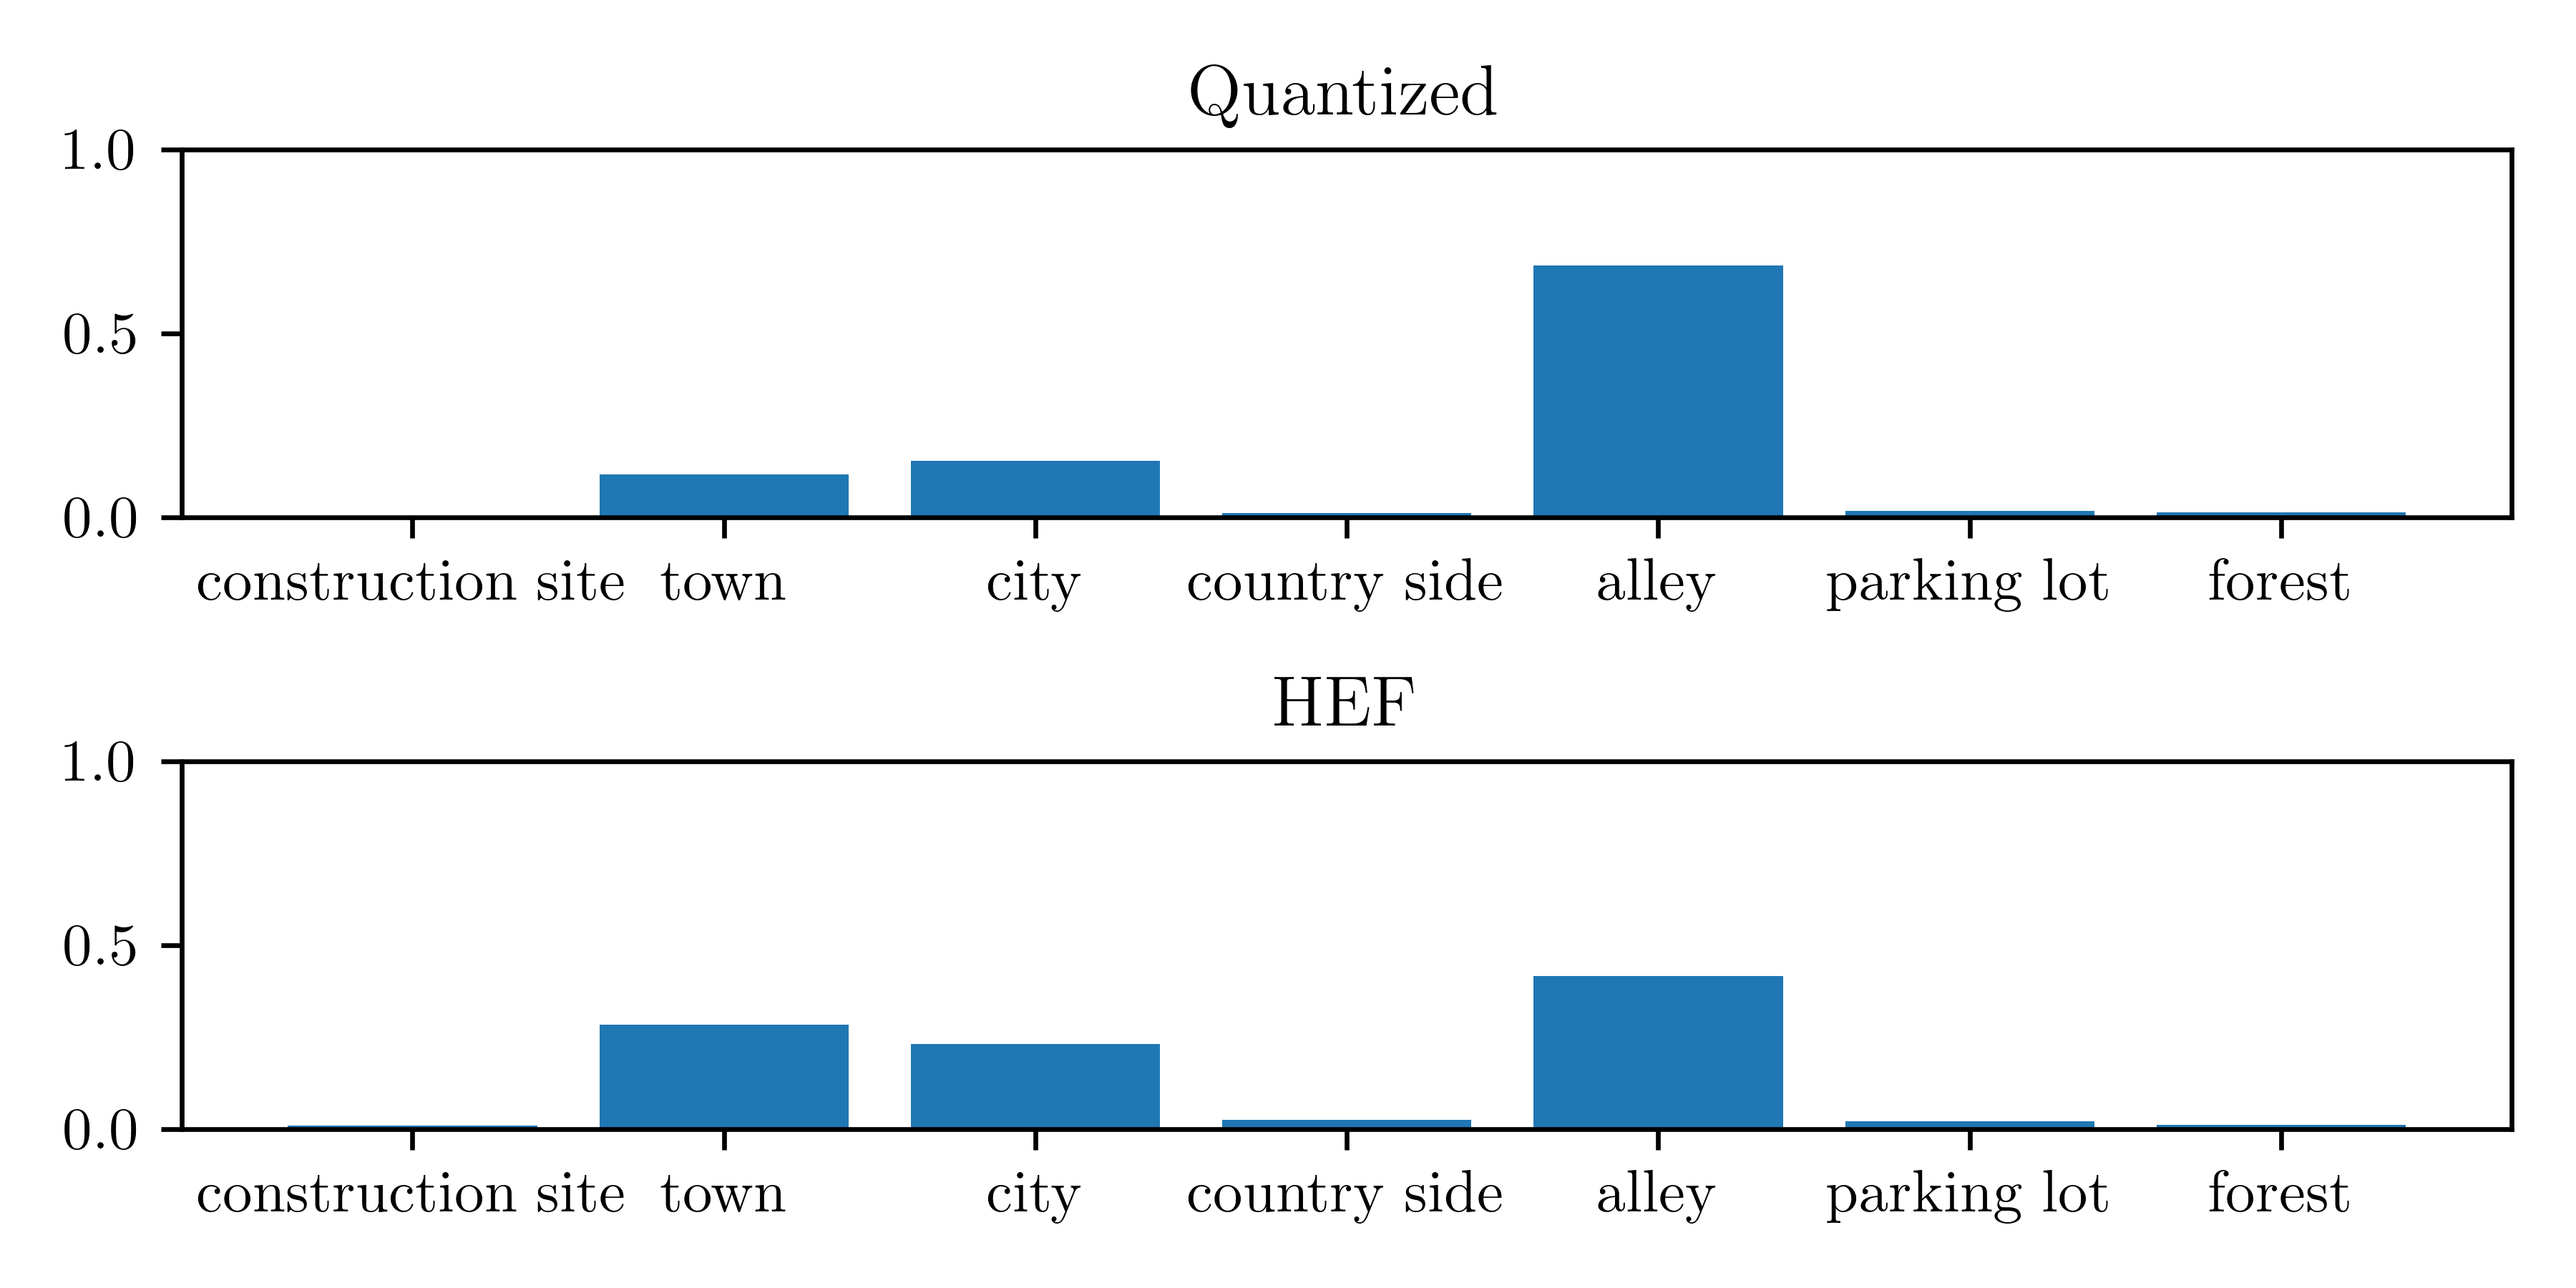
\includegraphics[width=0.75\textwidth]{Images/Implementation/compareProbs_RN50_quant_Hef.png}
    \caption{Testimage [panorama\_00002\_0014\_2] to compare outputs of Har quantized to \acrshort{hef}.}
    \label{methods:fig:comparern50harhef}
\end{figure}

\begin{figure}
    \centering
    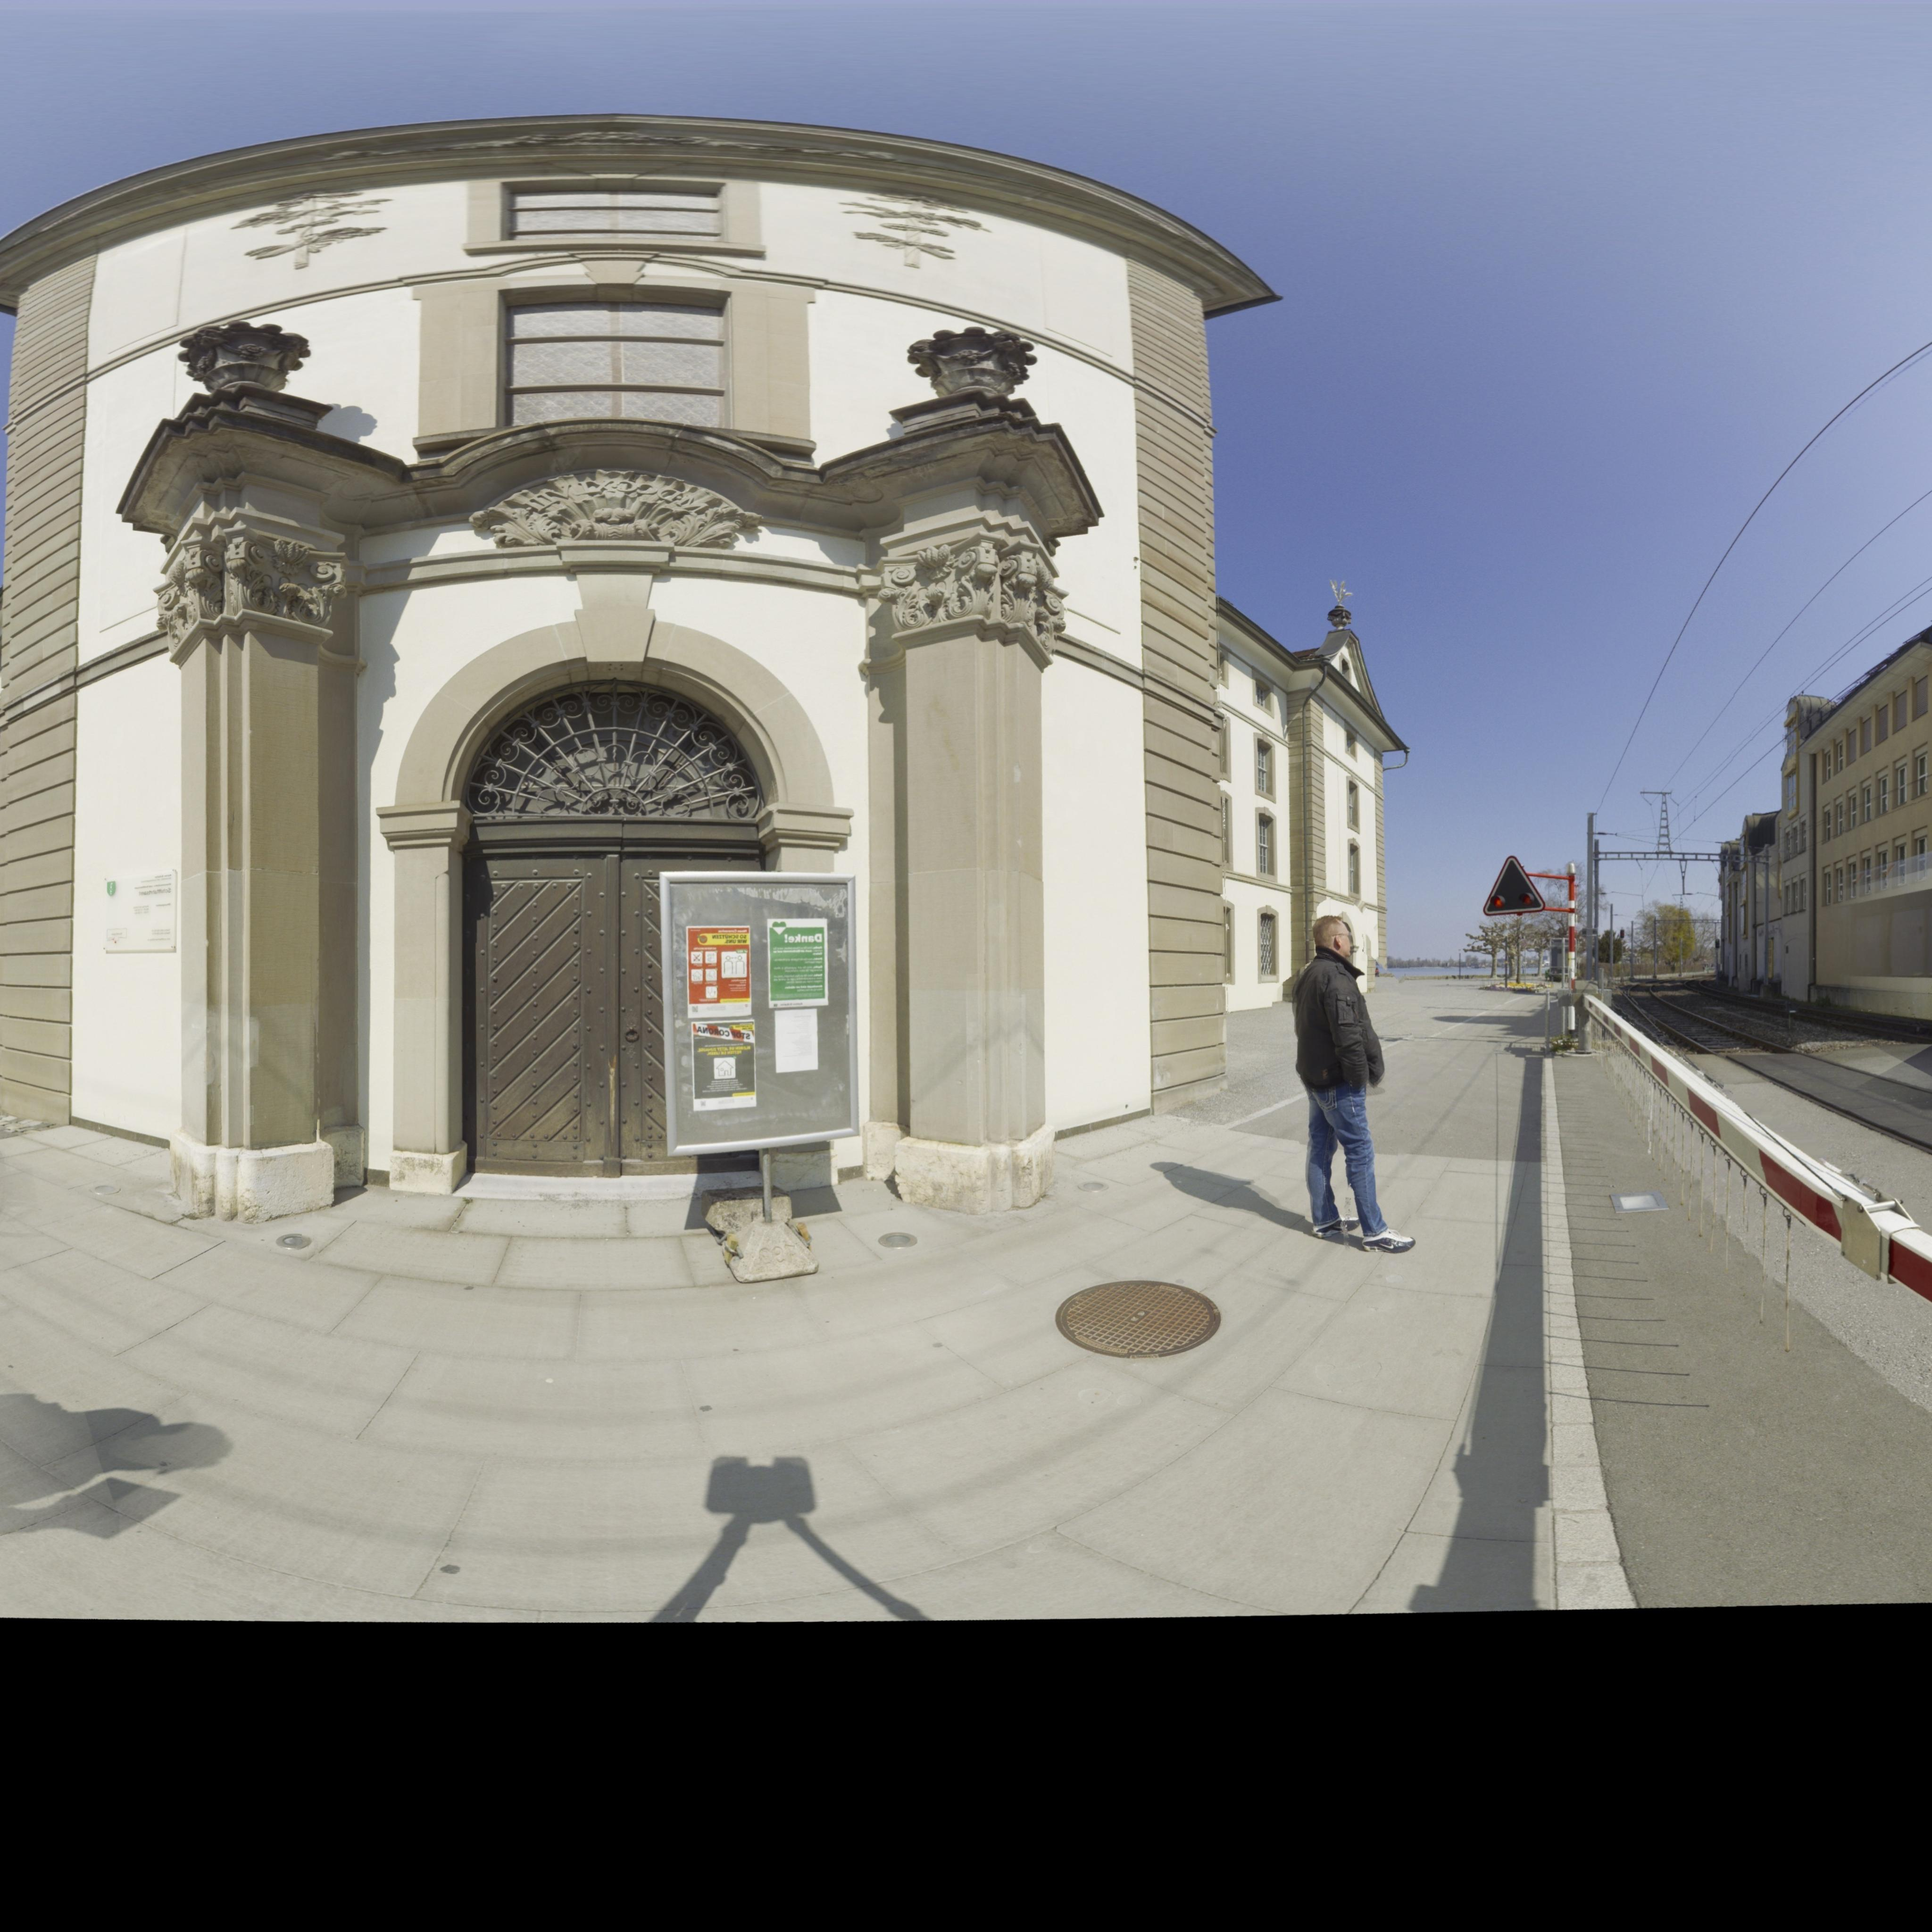
\includegraphics[width=0.5\textwidth]{Images/Implementation/panorama_00002_0014_2_testIMg.jpg}
    \caption{Testimage [panorama\_00002\_0014\_2] to compare outputs of the \acrshort{dfc}. The difference in the output is from changes to the architecture while compile \acrshort{har} to \acrshort{hef}.}
    \label{methods:fig:comparetestpic}
\end{figure}



\section{Increase accuracy}

Things mentiond in \cref{section:enhancealgorithm} would not make much sense to applied.
Most of the things mentiond extend the current network with some layers.
Due to the cutting of the network these layers have to be processed on the CPU of the Raspberry Pi which would decrease the throughput of the networks.
In \cref{scetion:methods:contimp} the reason for the bad accuracy is suspected to be the bad quantization.
The models are all translated to INT8.
In a attemp to increase accuracy as much as possible is converted to INT16.
Other ways to increase the accuracy are better text promts, adjusting the threshold for binary classifications or cutting the graph at a different position so that only operation which work well quantized are used on Hailo.

\subsection{Change the cut location
\label{methods:sec:cutlocation}}
A assumption is that the last part of the ResNet's, which is a self attention layer, is not quantizing propely due to some big matrix multipications.
To work against this effect the cut which in any case has to be made can appear earlier in the graph.
This means that only convolutions and additions were quantized and processed on hailo.
The cut location can be seen in \cref{methods:fig:rn50newcut}.

\begin{table}[]
    \centering
    \begin{tabular}{l|rrrrr}
        \hline
        Modelname & Accuracy &  \makecell{Balanced \\accuracy}&\makecell{Throughput\\(it/s)} & \makecell{Throughput \\ Image (it/s)} & \\ \hline
        RN50 & 0.799 & 0.200 & 20.30 $\pm$ 1.44 & 24.00 $\pm$ 1.19  \\ 
        RN50x4 & 0.845 & 0.560 & 9.30  $\pm$ 0.33 & 9.75  $\pm$ 0.33\\
        RN101 & 0.833& 0.414 & 15.22 $\pm$ 0.73 & 16.59 $\pm$ 0.49\\  
        TinyCLIP-19M & 0.175 & 0.217 & 28.40 $\pm$ 2.85 & 36.58 $\pm$ 3.38 \\ 
        TinyCLIP-30M & 0.625 & 0.426 & 21.61$\pm$ 1.35 & 23.84 $\pm$ 4.85\\ 
    \end{tabular}
    \caption{Performance table from evalutaion on Hailo-8L where the model graph is cut in a different location.}
    \label{methods:tab:perfHailocut}
\end{table}

In \cref{methods:tab:perfHailocut} that some models have a increased  in their accuracy some have a decrease in accuracy.
This means that no statment can be made about the new cut location.
The decrease in throughput is explained by a larger part which has to be calculated on the CPU.

\subsection{Adjust threshold}

A way to increase accuracy is to adjust the threshold.
This only works in binary classification.
This can be applied to the classification between indoor and outdoor and indoor construction and architectural.
For the outdoor classes (forest,urban and out construction) nothing like this can be done to increase the accuracy.
This threshold has to be calculate.
For this calculation one has to watch out to use a balanced dataset.
To get a balanced dataset a subset is created so that each class has the same amount of images.
The images are randomly sampled.
This process proved beneficial because it does not need much computational resources and its easily implemented.
Due to time limitations it was only applied to the classification between Indoot and Outdoor.
The result showed a small improvement.
The result can be seen in \cref{methods:tab:perfHailocutTh}.

\begin{table}[]
    \centering
    \begin{tabular}{l|rrr}
        \hline
        Modelname & Accuracy &  \makecell{Balanced \\accuracy}&  \makecell{Change in \\balanced accuracy}\\ \hline
        RN50 & 0.799 & 0.200  & 0\\ 
        RN50x4 & 0.845 & 0.560 & 0\\
        RN101 & 0.743& 0.507 & +0.93\\  
        TinyCLIP-19M & 0.141 & 0.211 & -0.06\\ 
        TinyCLIP-30M & 0.624 & 0.521 & +0.95\\ 
    \end{tabular}
    \caption{Performance table from evalutaion on Hailo 8L where the model graph is cut in a different location with calculated threshold .}
    \label{methods:tab:perfHailocutTh}
\end{table}


\begin{figure}[]
    \centering
    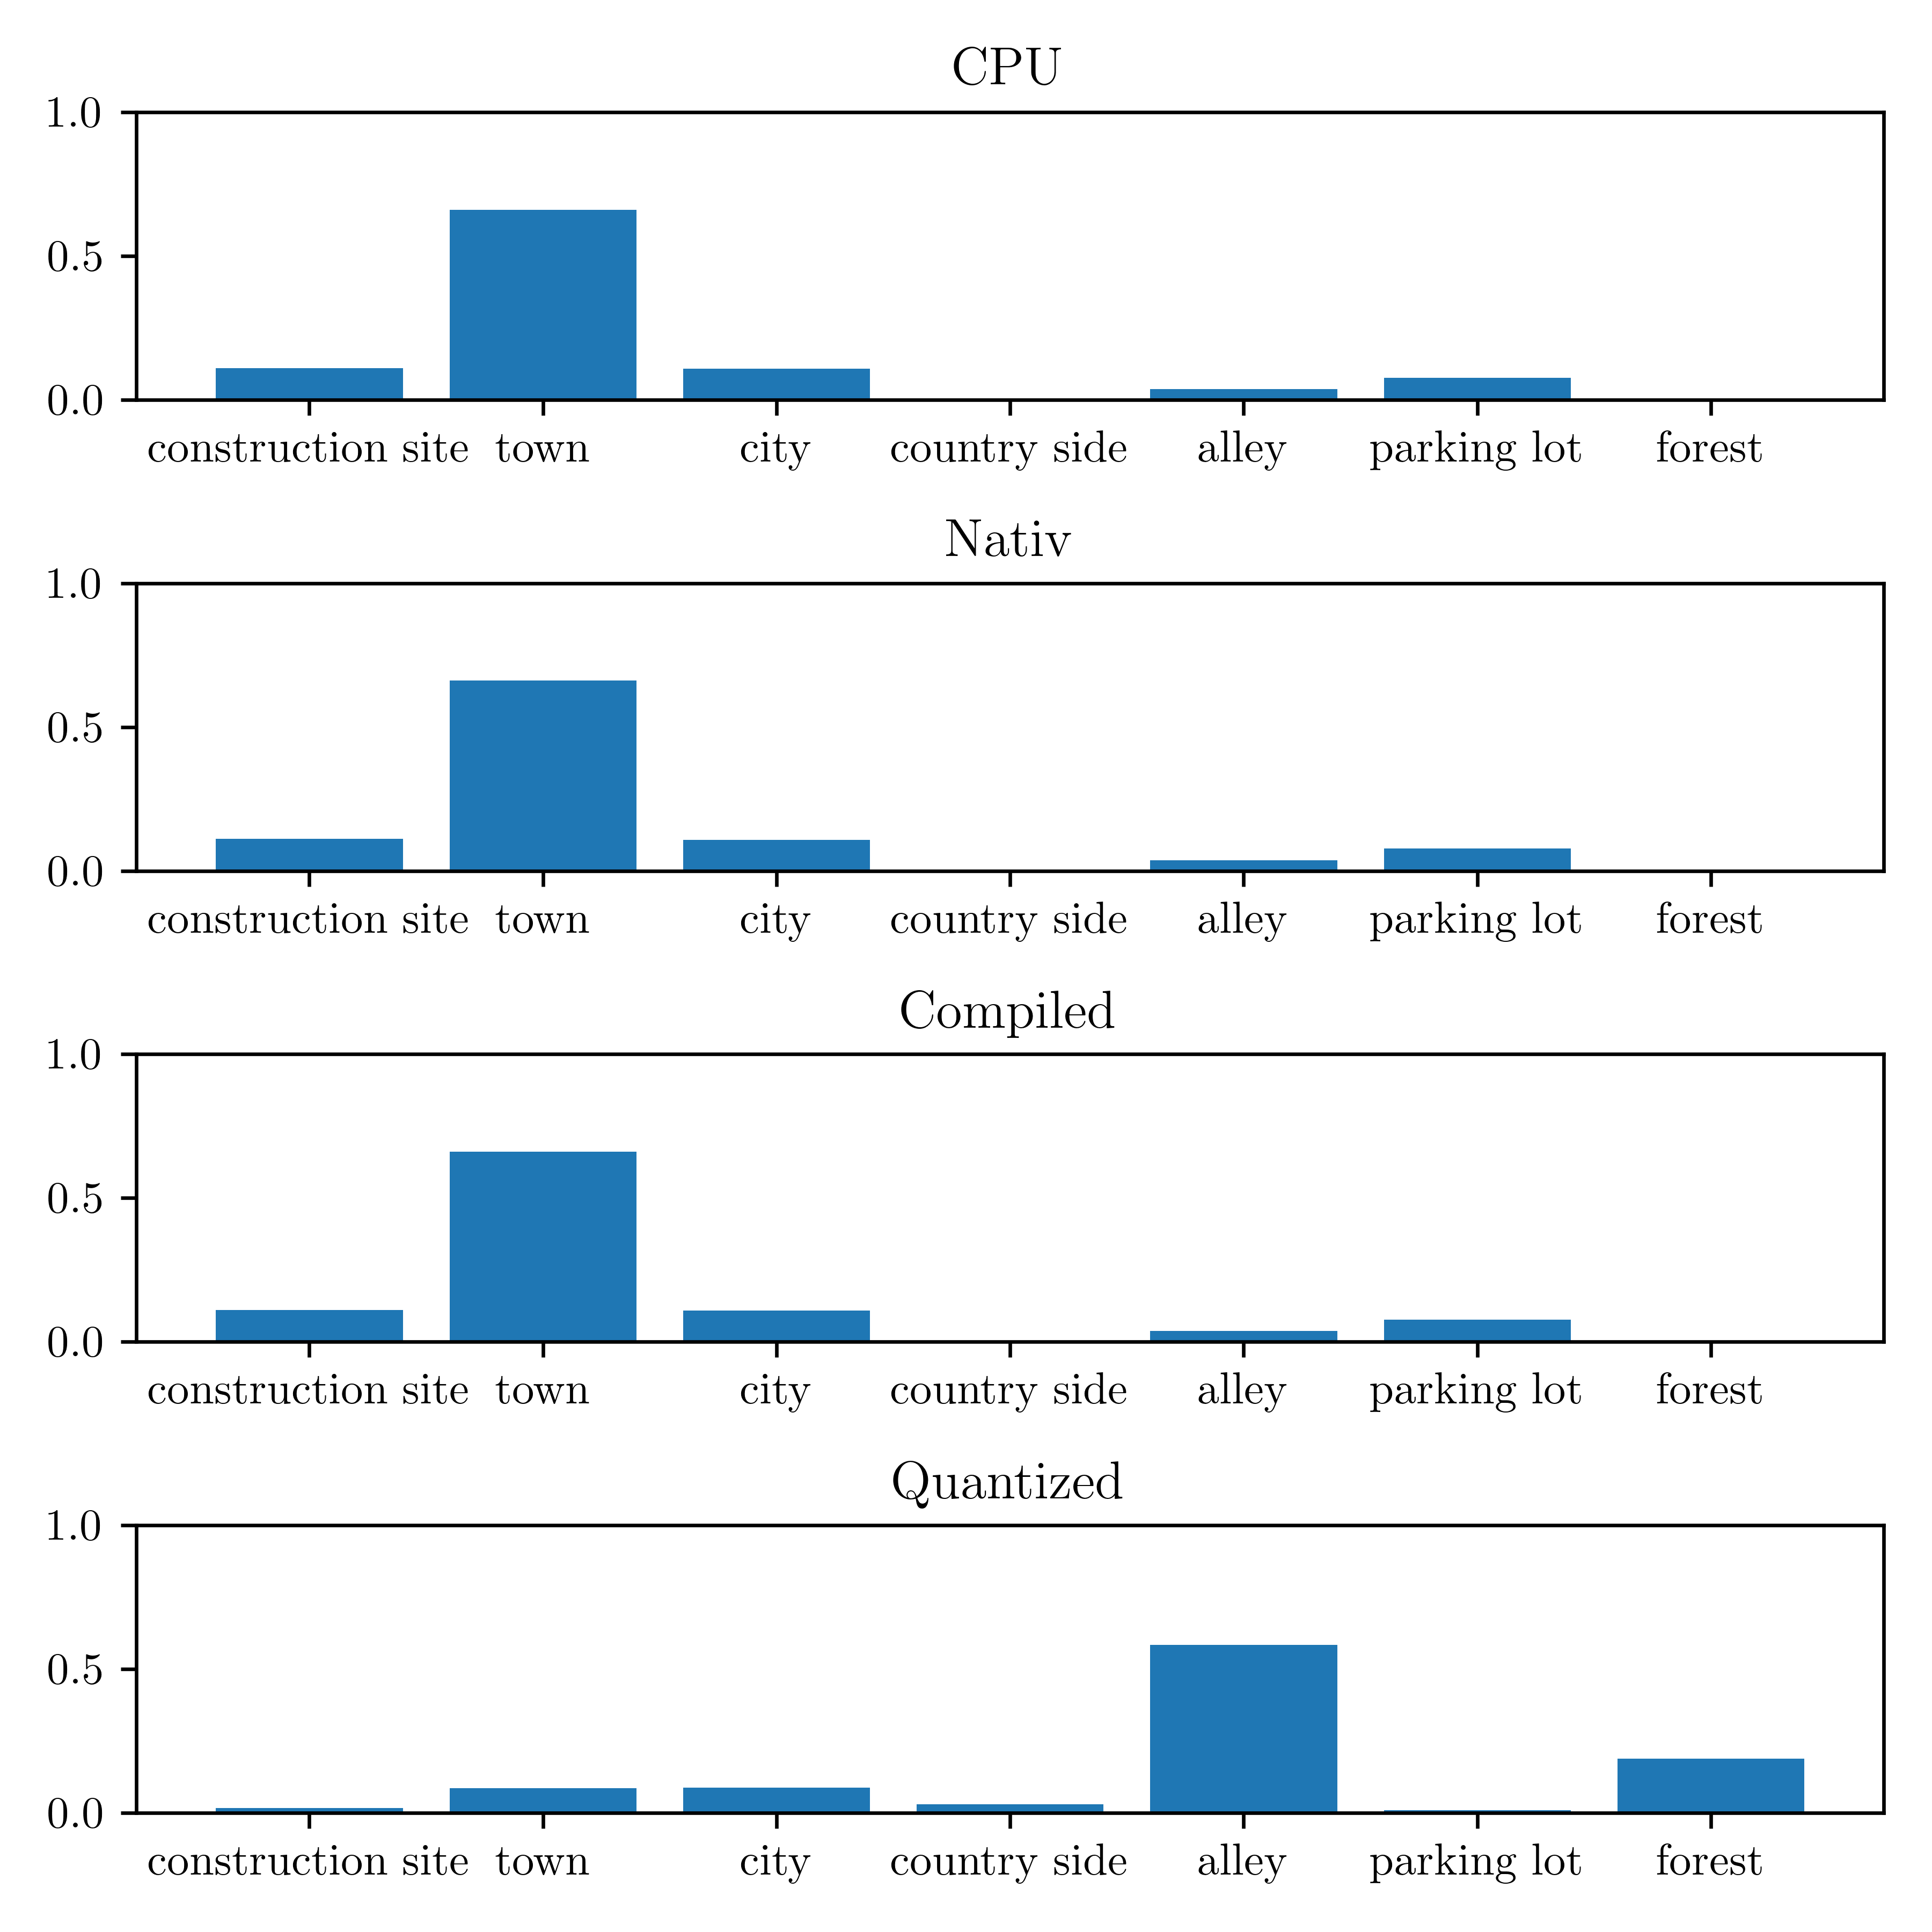
\includegraphics[width=0.6\textwidth]{Images/Implementation/compareProbs_newCut_RN50.png}
    \caption{Compare outputs at different \acrshort{dfc} points with RN50 with the new cut position. The new cut position showed no improvment when compared to \cref{methods:fig:comparern50}}
    \label{methods:fig:comparern50newcut}
\end{figure}

\begin{figure}[]
    \centering
    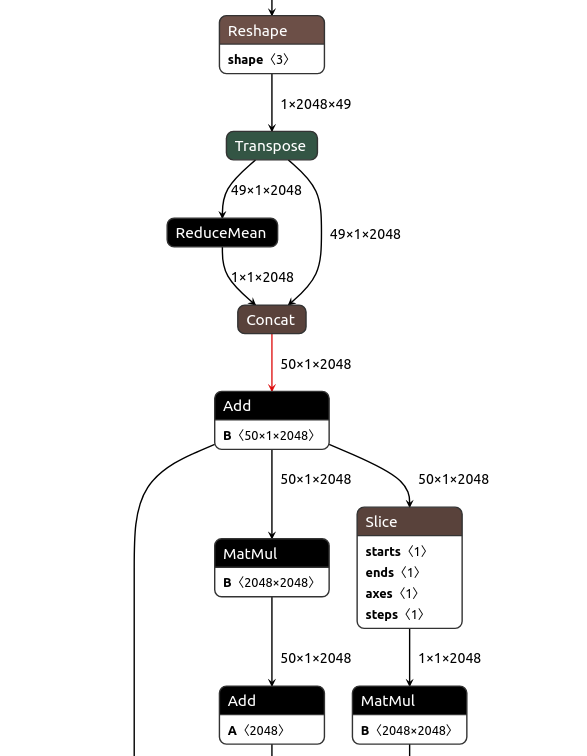
\includegraphics[width=0.4\textwidth]{Images/Implementation/secondcutlocation.png}
    \caption{Graph for the RN50. The new Cut location is at the red arrow between the Concat and the Add block.
    The location is similar for all models.}
    \label{methods:fig:rn50newcut}
\end{figure}

\subsection{Change quantization}

The \acrshort{dfc} offers a way to change the quantization of the weigths.
This is applied via the model script in quantization.
Due to the limitation that no GPU is available during the project quantizing a network to a different type than INT8 took very long.
Due to this reason only TinyCLIP-19M is quantized to INT16.
In the end 66\% of parameters were INT16 but no increase in accuracy was found.
Further test have to be made.
